\section{System architecure}
\label{sec:system_architecture}

\subsection{\SeeDB\ overiew}
\label{subsec:overview}

Figure \ref{fig:sys-arch} shows the architecture of our system. Currently,
\SeeDB\ is implemeted as a layer on top of a database. While optimization opportunities are
restricted by virtue of being outside the DBMS, it permits \SeeDB\ to be used 
with a variety of existing databases.

\begin{figure}[htb]
\centerline{
\hbox{\resizebox{9cm}{!}{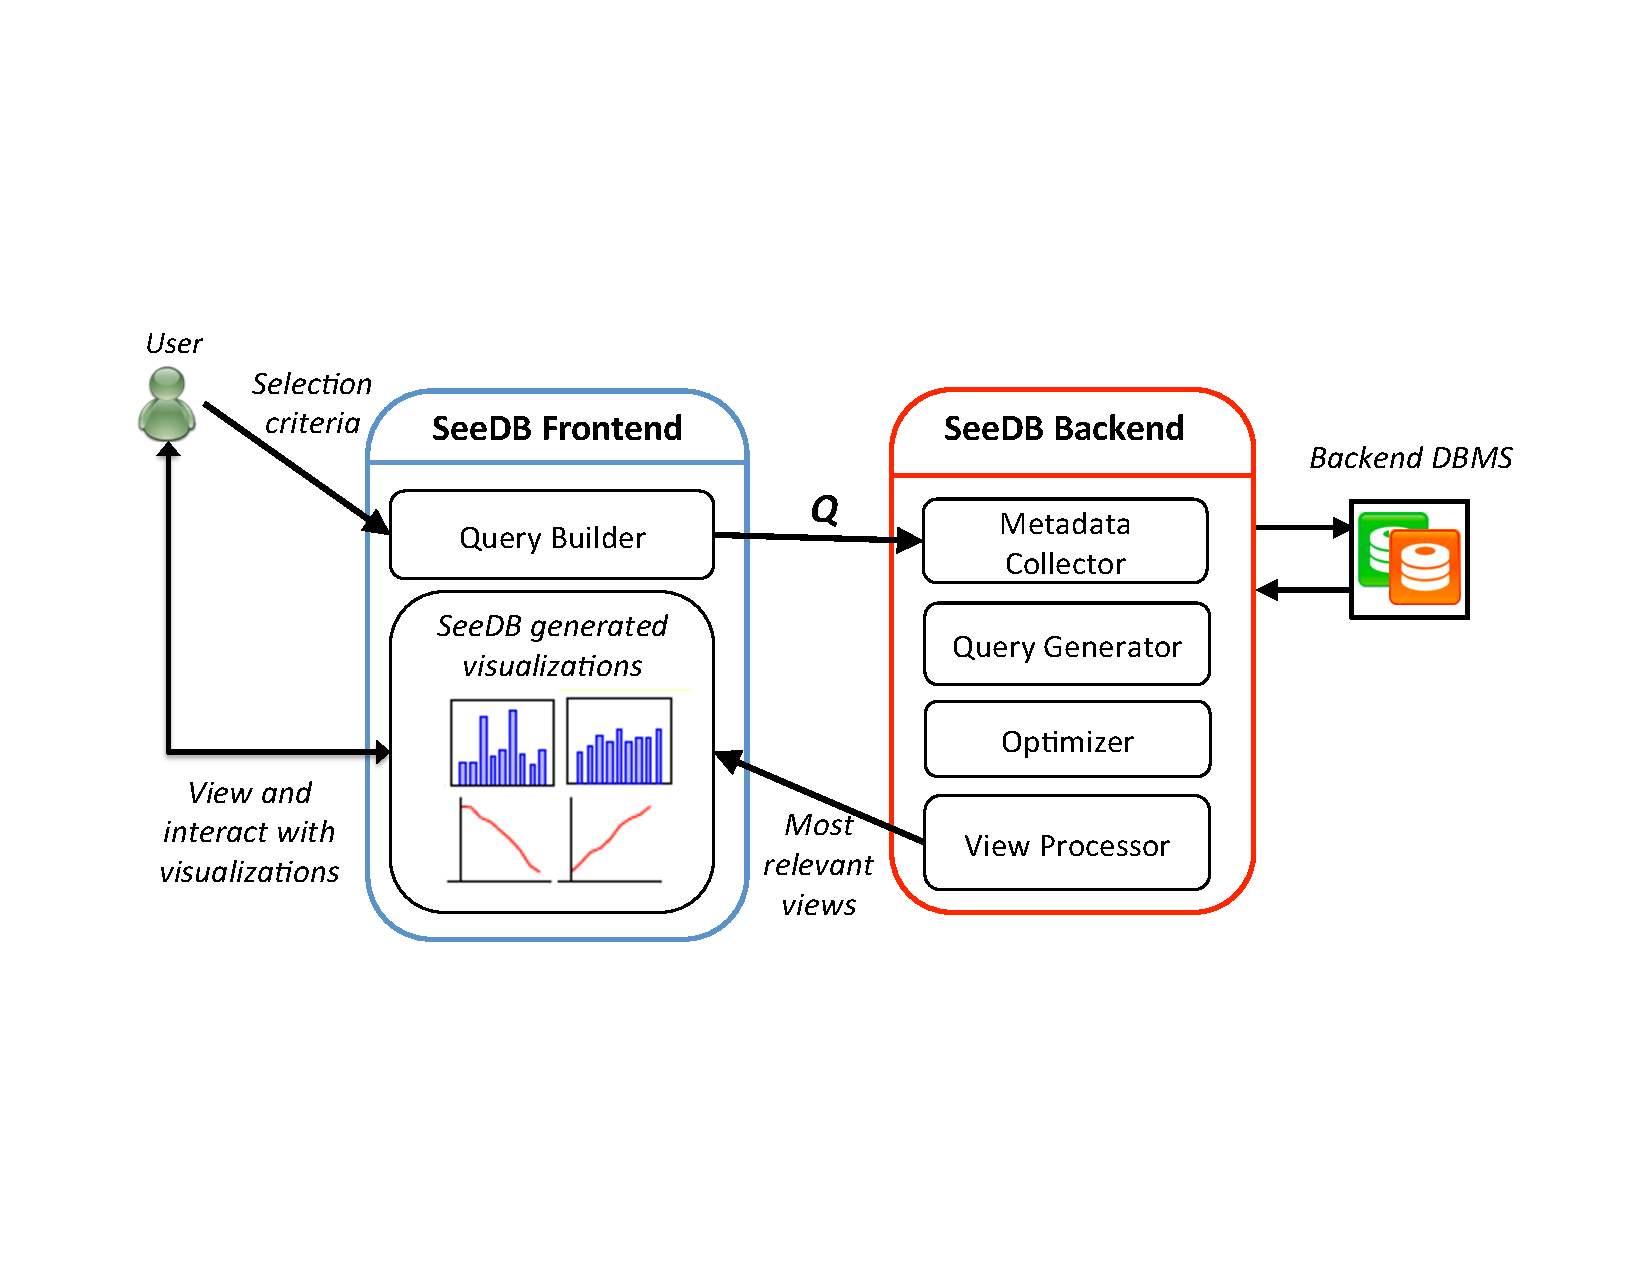
\includegraphics[trim=10mm 50mm 10mm 50mm,
clip=true]{Images/seedb-architecture.pdf}}}}
\caption{SeeDB Architecture}
\label{fig:sys-arch}
\end{figure} 

The \SeeDB\ front end allows the user to issue queries
through several means including raw SQL, via a query-builder and via
pre-formulated queries (more in Section \ref{subsec:seedb_frontend}). Once user
queries are sent to the backend, the Metadata Collector queries the relevant
tables for information such as table sizes, column types, table statistics etc.
This metadata is essential for the subsequent processing performed by \SeeDB\ .
The user queries along with metadata are then sent to the Query Generator.
The purpose of the Query Generator is two-fold: first, it uses the metadata and
user query to knock down the search space of possible view queries, and second,
it generates the remaining view queries that must be run against the databse.
The Optimizer is responsible for determining the best ways to combine view
queries so that total query execution time is minimized. We discuss some of the
optimizations performed by the Query Generator and Optimizer in Section
\ref{subsec:seedb_backend}. With the optimized queries in hand, \SeeDB\ asks the
DBMS to execute queries and return result to the View Processor that ingests
combined query results in a streaming fashion and produces results for
individual queries. The View Processor is also responsible for selecting the
most interesting views and returning them to the user.

\subsection{SeeDB Frontend}
\label{subsec:seedb_frontend}

The \SeeDB\ frontend has a two-fold purpose: allow the user to input a query, and 
to visualize
and analyze the resulting views. We provide the user with three options for
specifying an input query: (a) as raw SQL, (b) through a query builder that can
allow users unfamiliar with SQL to formulate queries through an easy-to-use
form-based interface, (c) through pre-defined query templates, e.g., queries
that select outliers in a particular column. These templates are particularly
useful since users are interested in anomalous data points.

Once a user submits a query to \SeeDB\, the \SeeDB\ engine evaluates various
views and sends the most promising ones to the frontend. The frontend then
determines the best ways to visualize these views (e.g. depending on data types
being represented and number of distinct values) and displays the
visualizations. The user can then examine these diverse views at a glance,
explore specific views in detail and view metadata for each view (e.g. size of
result, sample data, value with maximum change and statistics). The user can
also slice-and-dice views further by selecting particular values of grouping
attributes to explore. The user does this simply by selecting the relevant
attribute values in the view. This automatically modifies the selection query
and displays views for the subset of data selected. The user can of course
revert back to the original views and continue exploring the data.

\subsection{SeeDB Backend}
\label{subsec:seedb_backend}

One of the chief challenges in \SeeDB\ is producing the most interesting views
of the data in the minimum time. For this, \SeeDB\ must perform optimizations
at two stages: first, using prior knowledge such as statistics to prune out
uninteresting views without examining table data; and second, minimizing the
execution time for queries that are issued to the database. We first describe
the basic \SeeDB\ framework and then briefly discuss our optimizations.

\subsubsection{Basic Framework}
\label{subsubsec:basic_framework}

Given a user query $Q$, the basic version of \SeeDB\ computes all possible view
queries by adding a single aggregate and a single group-by clause to $Q$. Each
of these view queries is executed independently at the backend along with an
equivalent aggregate+group-by query on the complete underlying dataset. The two
resulting distributions are compared using the chosen distance metric (Section
\ref{sec:problem_statement}) and the top k views with the largest utility are
chosen. The frontend then visualizes the results. The basic approach is clearly 
inefficient and we can significantly improve performance.

\subsubsection{View Space Pruning}
\label{subsubsec:view_space_pruning}

To minimize the \SeeDB\ response time, we aggressively prune view queries that
are unlikely to generate interesting views. This pruning is based on prior
knowledge about the data as well as access patterns for the table (if
available). Specifically, we use variance estimates for table columns and
correlation measures between columns of the table. If two columns in the table
have high correlation, the views generated by grouping with respect to these two
columns will be very similar. We therefore only generate a single view for the
pair of columns. We can similarly use statistical properties of measure
attributes to prune views further. Finally, if access patterns for the table are
available, we can use them to prune views with attributes that are
rarely accessed and are therefore likely to be unimportant.

\subsubsection{View Query Optimizations}
\label{subsubsec:optimizations}

Since \SeeDB\ executes many similar queries, we clearly can do better than
the basic framework presented above, and \SeeDB\ implements various such
optimizations. Our optimization strategies include:

\begin{enumerate}
  \item {\it Rewrite view query}: Since similar group-by and aggregate queries
  are executed on the results of user query $Q$ and the underlying dataset,
  one straighforward optimization is to combine these two queries into one. 
  XXX actual queries.
  \item {\it Single Group-by Multiple Aggregates}: A large number of view
  queries have the same group-by clause but aggregates over different attributes.
  Therefore, \SeeDB\ combines all view queries with the same group-by clause
  into a single view query. This rewriting provides a speed up linear in the
  number of aggregate attributes.
  \item {\it Multiple Aggregate Computation}: 
  \SeeDB\ computes a large number of group-bys. One optimization is to
  combine queries with different group-by attributes into a single query with
  multiple group-bys attributes. For instance, consider view queries $V(Q,
  A_1,$ $G_1)$, $V(Q, A_1,$ $G_2)$ \ldots $V(Q, A_1,$ $G_n)$. Instead of
  executing them individually, we can rewrite them into a single view query
  $V(Q, A_1,$ $(G_1, G_2$\ldots $G_n))$. While this optimization can reduce the
  number of queries executed, the number of group by attributes we can include in a single query
  depends on the correlation between values of the various attributes (this
  affects number of distinct groups) and the working memory. We can compute the
  optimal combinations of group-bys by modeling the problem as a variant of
  bin-packing. 
%   A variation of this approach also implemented
%   on \SeeDB\ is to send the results of the multiple group-by query to the front
%   end and ask the \SeeDB\ frontend to compute utility and select views. The
%   advantage of this approach is that it allows for more efficient interactive
%   exploration of the views.
  \item {\it Sampling}: The optimization that can have the most impact in
  terms of efficiency is to reduce the number of tuples examined by
  constructing a data sample and running all queries against the sample. As
  expected, the sampling technique and size of the sample can affect the
  accuracy of the generated views. 
\end{enumerate}

%\begin{figure}[htb]
%\centerline{
%\hbox{\resizebox{9cm}{!}{\includegraphics[trim=10mm 50mm 10mm 50mm,
%clip=true]{Images/seedb-frontend.pdf}}}}
%\caption{SeeDB Frontend}
%\label{fig:frontend}
%\end{figure} 


